\chapter{Python图像处理}
\label{cp:pythonimage}

本部分的目标是\textbf{通过使用Python中的多个库,理解图像处理的基本概念和操作}。我们\textit{并不指望通过一次实验就对所有技术都掌握},只希望通过实际的代码示例与实验,逐步了解图像的\textit{格式转换、图像显示、灰度变换、图像模糊处理}等核心技术,为后续可能的深入学习、和其他更加高深的如机器学习和深度学习中的图像处理奠定基础。

\section{使用PIL库处理图像}

\subsection{PIL库简介}

\textbf{Python Imaging Library (PIL) 是用于图像处理的Python库}。提供了许多通用的功能,包括\textit{图像的读取、处理和保存}。\\

由于PIL库的开发已经停止,我们将\textbf{使用其继承库Pillow}。\texttt{Pillow}是PIL库的一个分支,\textit{支持Python3},而PIL库只支持Python2。\\

本次实验中,我们将使用PIL进行\textit{图像格式的转换、创建缩略图以及复制粘贴图像区域}等基本操作。

\subsection{图像格式转换}
\label{subsec:formatconvert}

我们可以使用PIL加载图像文件并调用 \texttt{save()} 方法,轻松地将图像从一种格式转换为另一种格式。具体的代码实现如下:

\begin{longlisting}
    \begin{minted}{python}
from PIL import Image
import os

# 图像文件列表
filelist = ['image1.png', 'image2.bmp', 'image3.tiff']

# 输出目录
output_dir = './converted_images/'

# 确保输出目录存在
os.makedirs(output_dir, exist_ok=True)

# 遍历文件列表并将图像转换为 JPEG 格式
for infile in filelist:
    # 打开图像文件
    img = Image.open(infile)
    
    # 获取文件名和扩展名
    filename, _ = os.path.splitext(os.path.basename(infile))
    
    # 转换并保存为 JPEG 格式
    img.convert('RGB').save(os.path.join(output_dir, filename + '.jpg'), 'JPEG')

print("所有图像已成功转换为 JPEG 格式!")
    \end{minted}
    \caption{使用PIL转换图像格式}
    \label{listing:pilconvert}
\end{longlisting}

我们首先导入了 \texttt{Image} 类,然后定义了一个图像文件列表 \texttt{filelist} 和一个输出目录 \texttt{output\_dir}。接着,我们遍历文件列表,打开每个图像文件并将其转换为JPEG格式,最后保存到输出目录中。\\

如图\ref{fig:pilconvert}所示,我们可以看到,原始的三个图像文件已经成功转换为JPEG格式。

\begin{figure}[!h]
    \centering
    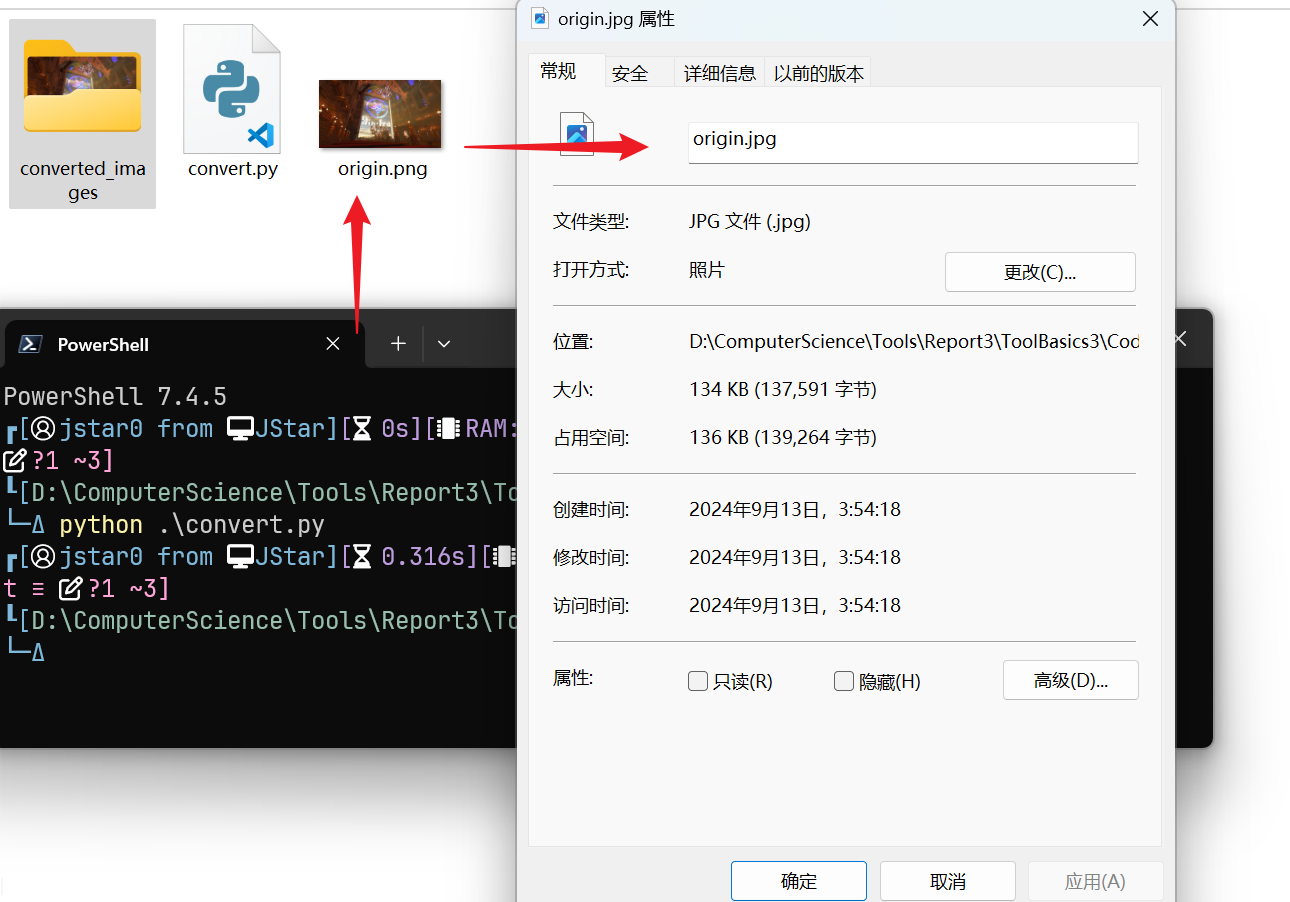
\includegraphics[width=.8\textwidth]{./Figures/PIL1.png}
    \caption{使用PIL转换图像格式}
    \label{fig:pilconvert}
\end{figure}

\subsection{创建缩略图}

\texttt{thumbnail()}方法可以用于\textbf{生成图像的缩略图},会\texttt{根据指定的尺寸自动缩放图像,保持宽高比}。缩略图操作将直接在原始图像对象上进行,不会返回新的图像对象。具体的代码实现如下:

\begin{longlisting}
    \begin{minted}{python}
from PIL import Image
import os

# 图像文件列表
filelist = ['image1.jpg', 'image2.jpg', 'image3.jpg']

# 输出目录
output_dir = './thumbnails/'

# 缩略图的最大尺寸
size = (128, 128)

# 确保输出目录存在
os.makedirs(output_dir, exist_ok=True)

# 遍历文件列表并生成缩略图
for infile in filelist:
    # 打开图像文件
    img = Image.open(infile)
    
    # 生成缩略图
    img.thumbnail(size)
    
    # 获取文件名
    filename = os.path.basename(infile)
    
    # 保存缩略图
    img.save(os.path.join(output_dir, filename))

print("缩略图已成功生成!")
    \end{minted}
    \caption{使用PIL生成缩略图}
    \label{listing:pilthumbnail}
\end{longlisting}

同\nameref{subsec:formatconvert}一样,具体内容就不加赘述了。

\section{使用Matplotlib库显示图像}

该库由于我在数学建模时有所接触,所以这里就不再赘述了。为您呈现一个数学建模时正好用到的代码:

\begin{longlisting}
    \inputminted{python}{./Codes/Matplotlib/1.py}
    \caption{使用Matplotlib绘制“板凳龙”}
    \label{listing:benchdragon}
\end{longlisting}

该代码由我们小组共同完成,绘制了\textit{“板凳龙”在盘入时的约定的t时刻上,板凳的把手的位置,底图是一个阿基米德螺线}。最终得到的图像如\autoref{fig:benchdragon}所示。\\

我们的代码提供了一个真实的样例,那就是通过\texttt{Matplotlib}库,可以通过数学方法,便捷地绘制出复杂的图像。此外,本文档还用到了\texttt{numpy, scipy}库,用于处理数学运算。\\

\begin{figure}[!h]
    \centering
    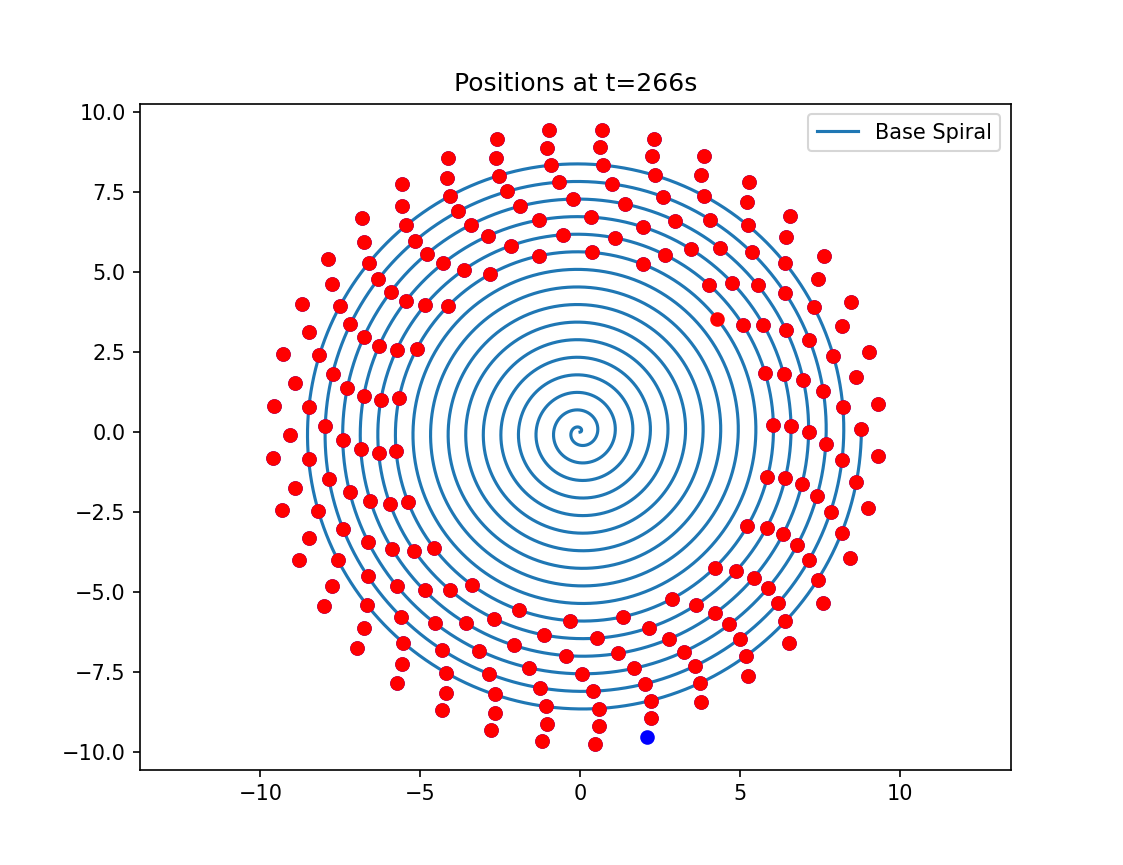
\includegraphics[width=.8\textwidth]{./Figures/M.png}
    \caption{“板凳龙”在盘入时的t=166s时刻上,板凳的把手的位置}
    \label{fig:benchdragon}
\end{figure}

\section{学习NumPy进行图像处理}

由于内容的复杂和专业性,该部分的内容查阅了相关的资料,包括但不限于\cite{solem2014python计算机视觉编程}。原理复杂,仅作为学习笔记。

\subsection{灰度转换}

图像处理中,\textit{灰度图像是指每个像素点只包含亮度信息,而不包含颜色信息。}经查,\textit{灰度值可以通过将RGB三个颜色通道的值进行加权平均或简单平均得到}。NumPy可以直接操作图像的像素值,完成彩色图像到灰度图像的转换。\\

常见的灰度转换公式是:
\[
\text{Grayscale} = 0.2989 \times R + 0.5870 \times G + 0.1140 \times B
\]

藉由此公式,我们可以给出一个模板程序,实现如下:

\begin{longlisting}
    \begin{minted}{python}
import numpy as np
from PIL import Image

# 打开彩色图像
color_image = Image.open('color_image.jpg')

# 将图像转换为NumPy数组
image_array = np.array(color_image)

# 检查图像模式,如果不是RGB模式则转换为RGB模式
if color_image.mode != 'RGB':
    color_image = color_image.convert('RGB')

# 提取RGB通道
r, g, b = image_array[:,:,0], image_array[:,:,1], image_array[:,:,2]

# 上述公式
gray_image = 0.2989 * r + 0.5870 * g + 0.1140 * b

# 将灰度图像转换回PIL图像并保存
gray_image_pil = Image.fromarray(np.uint8(gray_image))
gray_image_pil.save('grayscale_image.jpg')

print("彩色图像已成功转换为灰度图像!")
    \end{minted}
    \caption{使用NumPy进行灰度转换}
    \label{listing:npgray}
\end{longlisting}

转换的成果如\autoref{fig:npgray}所示。

\begin{figure}[!h]
    \centering
    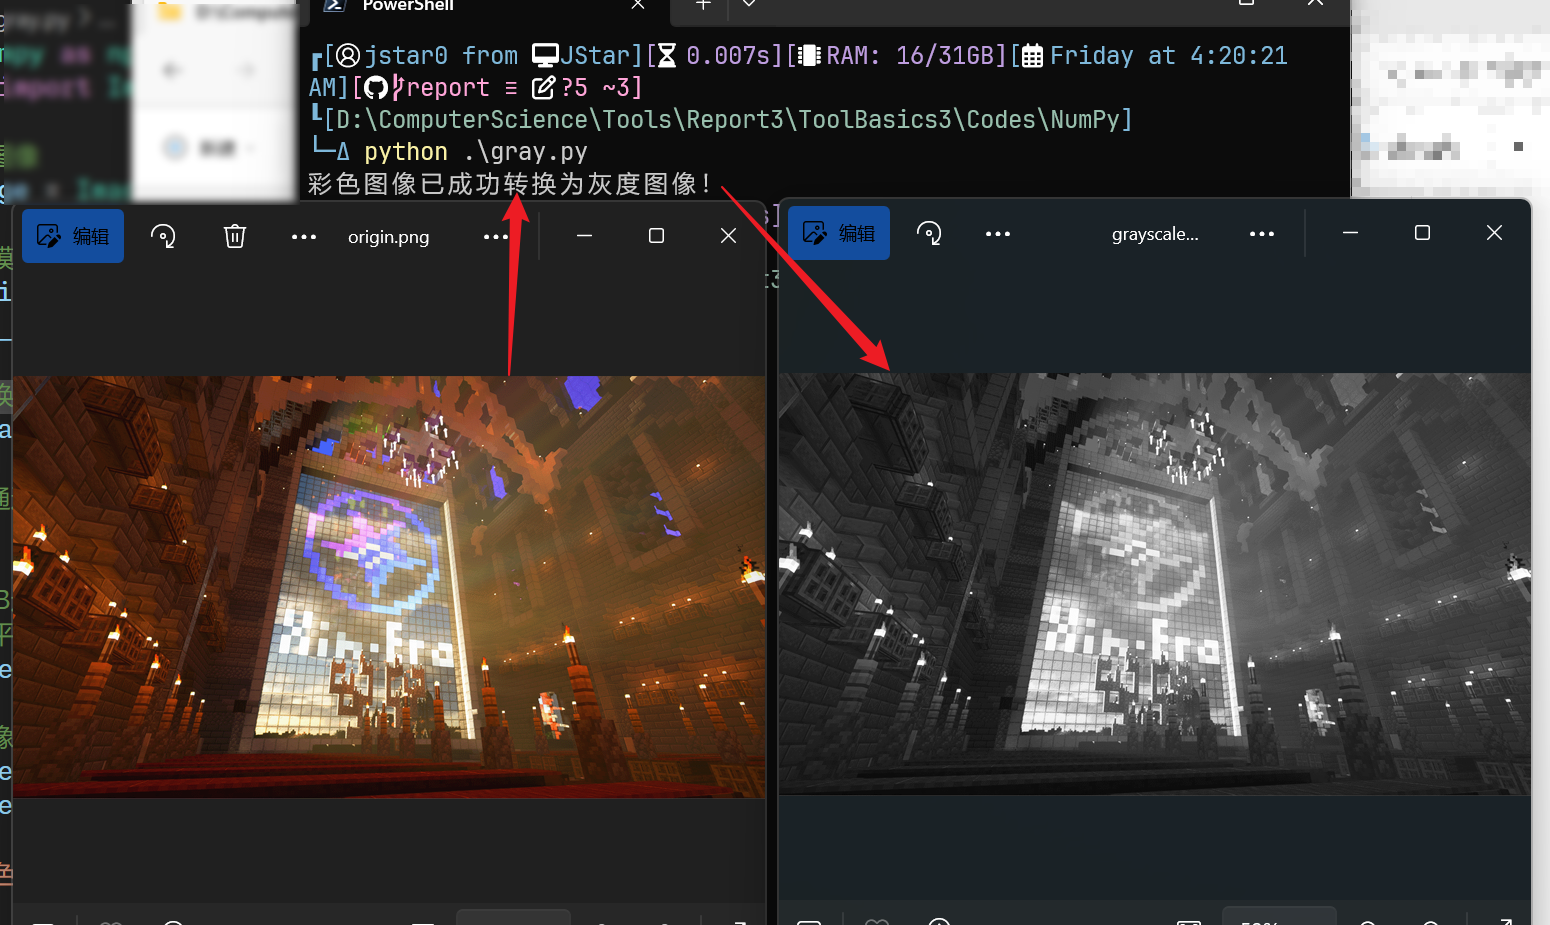
\includegraphics[width=.8\textwidth]{./Figures/N1.png}
    \caption{使用NumPy进行灰度转换}
    \label{fig:npgray}
\end{figure}

\subsection{直方图均衡化}

这部分的内容参考了\cite{solem2014python计算机视觉编程}及\cite{天海一直在AI2022}。\textit{直方图均衡化是一种用于增强图像对比度的技术}。它通过\textit{重新分布图像的像素值},使得图像的直方图更加均匀,从而增强图像的对比度。\\

由于篇幅限制,只得给出一个模板程序,实现如下:

\begin{longlisting}
    \begin{minted}{python}
import numpy as np
from PIL import Image
import matplotlib.pyplot as plt

# 打开灰度图像
gray_image = Image.open('grayscale_image.jpg')

# 将图像转换为NumPy数组
image_array = np.array(gray_image)

# 计算图像的直方图
hist, bins = np.histogram(image_array.flatten(), 256, [0, 256])

# 计算累计分布函数(CDF)
cdf = hist.cumsum()

# 将CDF进行归一化
cdf_normalized = cdf * hist.max() / cdf.max()

# 使用线性插值的方式进行直方图均衡化
cdf_m = np.ma.masked_equal(cdf, 0)
cdf_m = (cdf_m - cdf_m.min()) * 255 / (cdf_m.max() - cdf_m.min())
cdf = np.ma.filled(cdf_m, 0).astype('uint8')

# 应用CDF到原始图像
equalized_image = cdf[image_array]

# 将均衡化后的图像保存并显示
equalized_image_pil = Image.fromarray(equalized_image)
equalized_image_pil.save('equalized_image.jpg')

# 显示对比图
plt.figure()
plt.subplot(1, 2, 1)
plt.title('Original Image')
plt.imshow(gray_image, cmap='gray')

plt.subplot(1, 2, 2)
plt.title('Equalized Image')
plt.imshow(equalized_image_pil, cmap='gray')

plt.show()

print("图像的直方图均衡化已成功完成!")
    \end{minted}
    \caption{使用NumPy进行直方图均衡化}
    \label{listing:npequalize}
\end{longlisting}

成果如\autoref{fig:npequalize}所示。

\begin{figure}[!h]
    \centering
    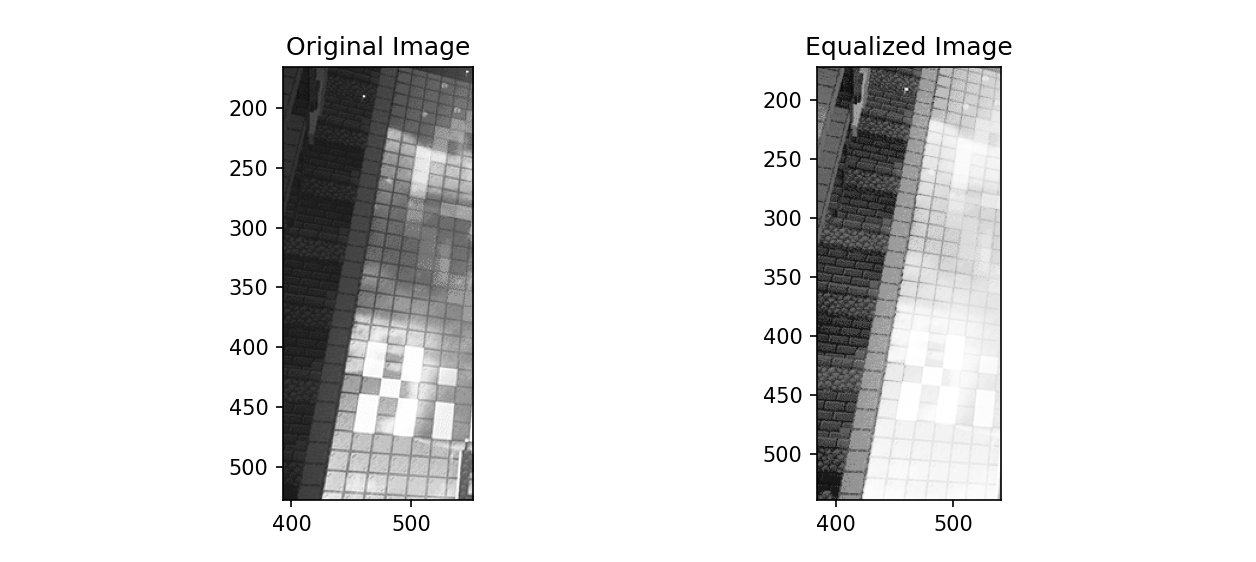
\includegraphics[width=.8\textwidth]{./Figures/N2.png}
    \caption{使用NumPy进行直方图均衡化}
    \label{fig:npequalize}
\end{figure}

\subsection{主成分分析 (PCA)}

\textbf{主成分分析 (PCA) 是一种降维技术,常用于图像处理中,以减少图像的冗余信息。}使用这种办法,我们可以\textit{将图像从高维空间投影到一个低维空间,保留大部分重要信息,同时降低图像数据的维度。}\\

由于我实在粗浅,只得使用封装好的库\texttt{sklearn.decomposition.PCA}实现主成分分析。示例代码如下:

\begin{longlisting}
    \begin{minted}{python}
import numpy as np
from PIL import Image
from sklearn.decomposition import PCA
import matplotlib.pyplot as plt

# 打开灰度图像
gray_image = Image.open('grayscale_image.jpg')

# 将图像转换为NumPy数组
image_array = np.array(gray_image)

# 将2D图像数组转换为1D数组
image_reshaped = image_array.reshape(-1, 1)

# 使用PCA进行降维
pca = PCA(n_components=50)  # 保留50个主成分
pca_result = pca.fit_transform(image_reshaped)

# 将降维后的图像重构回2D
image_reconstructed = pca.inverse_transform(pca_result).reshape(image_array.shape)

# 将结果转换为8位图像并保存
image_pca_pil = Image.fromarray(np.uint8(image_reconstructed))
image_pca_pil.save('pca_image.jpg')

# 显示原图和PCA降维后的图像
plt.figure()
plt.subplot(1, 2, 1)
plt.title('Original Image')
plt.imshow(gray_image, cmap='gray')

plt.subplot(1, 2, 2)
plt.title('PCA Image')
plt.imshow(image_pca_pil, cmap='gray')

plt.show()

print("图像的PCA降维已成功完成!")
    \end{minted}
    \caption{使用NumPy进行主成分分析}
    \label{listing:nppca}
\end{longlisting}

\subsection{使用SciPy进行数学运算}

相关的内容您可以参看\nameref{listing:benchdragon},这里面由用到\texttt{SciPy}的\texttt{fsolve}函数,用于求解非线性方程组。\\

\section{小结}

本次我们通过实践,深入了解了如何使用Python中的\emph{PIL、NumPy、Matplotlib和SciPy等库},完成了图像处理的多个核心操作,\textbf{转换了图像的格式、生成了缩略图、将彩色图像转换为灰度图像、进行了直方图均衡化、实现了主成分分析}等操作。\\

我们对图像处理的基本概念和操作积累了更深入的了解,为今后的学习和研究打下了基础。